%===================================== CHAP 4 =================================

\chapter{Test cases and results}

\begin{itemize}
    \item Aim of section ect...
\end{itemize}

In this project the test cases are based on a simple model with two neurons, $N_1$ and $N_2$. $N_1$ has for each time step a constant probability for spiking that depends on some background rate $b_1$. $N_2$ has spiking probability that depends on the spiking of $N_1$ in the previous time step through $b_2 + w_{21}(t) \cdot s_1(t_{j-1})$. So now we have,

\begin{align*}
    s_1(t) \sim \text{Ber}(\pi_1(t)) && \pi_1(t)= \frac{1}{1+exp(-b_1)} \\
    s_2(t) \sim \text{Ber}(\pi_2(t)) && \pi_2(t)= \frac{1}{1+exp(-(b_2 + w_{21}(t) \cdot s_1(t-1)))}
\end{align*}

For the test cases the parameter values to be used are $b1 = 0.5$ and $b2 = 0$. This corresponds to a background firing rate of 0.62 and 0.5 for neuron 1 and 2 respectively. The value for the weight $w_{12}$ will be let to vary with time, but a typical size for it will be $w_{12}=0.7$. This gives a value of 1.2 for the linear predictor when neuron 1 spiked in the previous time step, and a corresponding firing rate of 0.77 for neuron 2.

\begin{itemize}
    \item Maybe a small illustration?
\end{itemize}

\subsection{Precalculations}

\begin{itemize}
    \item The aim here is to calculate how well I expect my tests to work. Can use hypothesis testing on bernoulli GLM 
    \item Say something about how many time points ect that is needed to be able to detect a change of the weights
\end{itemize}

\begin{wraptable}{r}{4cm}
\begin{center}
 \begin{tabular}{||c c c ||} 
 \hline
 n & Lower & Upper \\ [0.5ex] 
 \hline\hline
 10 & 0.5 & 1 \\ 
 \hline
 100 & 0.7 & 0.84 \\
 \hline
 1000 & 0.748 & 0.792 \\
 \hline
 10000 & 0.7631 & 0.7769 \\ [1ex] 
 \hline
\end{tabular}
\end{center}
\end{wraptable}

\begin{figure}[h]
    \centering
    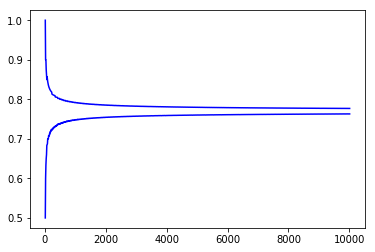
\includegraphics[scale=0.7]{Conf_intervals.png}
\end{figure}

It is practical to have some understanding of how precisely the weights can be inferred from the spike data. When performing $n$ repeated trials of a Bernoulli process with success rate $\pi$, the sum successes comes from a binomial distribution, with parameters $n$ and $\pi$. For some success count, $n_{success}$, the parameter $\pi$ can be estimated as $\frac{n_{success}}{n}$. How good this estimate is depends on the number of trials, $n$. Figure ?? and table ?? presents the endpoints of range that contains 90\% of the distribution, for different values of n (scaled by one over n). 
 %A simple toy example for illustration is a network consisting of two neurons, $N_1$ and $N_2$. $N_1$ has for each time step a constant probability for spiking that depends on some background rate $b_1$. $N_2$ has spiking probability that depends on the spiking of $N_1$ in the previous time step through $b_2 + w_{21}(t) \cdot s_1(t_{j-1})$, where $w_{21}(t)$ is some weight function. This can be modelled by Bernoulli GLMs where the variables $s_1(t_j)$ and $s_2(t_j)$ come from Bernoulli distributions, with probability parameters $\lambda_i(t)$ calculated from the linear predictors through a logit link function. The model can be summed up as follows 

%\begin{align*}
    %s_1(t) \sim \text{Bernoulli}(\lambda_1(t)) && \lambda_1(t)= logistic(b_1) \\
    %s_2(t) \sim \text{Bernoulli}(\lambda_2(t)) && \lambda_2(t)= logistic(b_2 + w_{21}(t) \cdot s_1(t_{j-1}))
%\end{align*}

%Both $b_2$ and $w_{12}(t)$ are unknown parameters, and the goal is to determine the values for them that gives the maximum likelihood for the observed data. To begin with, let $w_{12}(t)=w_{12}$. This gives a convex problem that can be solved using gradient ascent.

%When $w_{12}$ is allowed to vary with time, the problem is not necessarily convex anymore so gradient ascent is not applicable. To overcome the problem, the next step is to sample from the posterior distribution using Markov chain Monte Carlo techniques. 
\subsection{Constant weight}

\begin{itemize}
    \item Inferring constant weight using gradient ascent. Figure
    \item Inferring constant weight with Metropolis-Hastings
\end{itemize}

\subsection{Inferring dynamic weights}
Now the weights are let to vary. This makes the number of unknown parameters change from one to $T$. As described in section ??, as the number of data points is the same as the number of parameters, we need to take advantage of prior knowledge to infer the weights. This section presents the investigation of inferring dynamic weights using the Metropolis-Hastings algorithm.

For all test cases in this section we consider the case of having $T=10$. The weight corresponding to $t_{10}$ is not interesting, as no spikes are generated by it. Therefore there are 9 weights to infer. The true weights used in the spike simulations are set by specifying the weight at $t=t_1$ to be 0.7, $W_{t_1}^0 = 0.7$. The remaining weight trajectory is drawn as the weight of the previous time step plus the absolute value of a normal distributed parameter with zero mean and variance equal to $0.001$. This is a unrealistic big variance. In reality the number of time steps is much larger, and changing much slower. However, it is chosen this way to easily gain insight into the issue of inferring varying weights. \\

\textsc{Starting iterations from true weights}\\
For the first case the true weight trajectory is plotted in the following figure. 


\begin{figure}[hbt!]
    \centering
    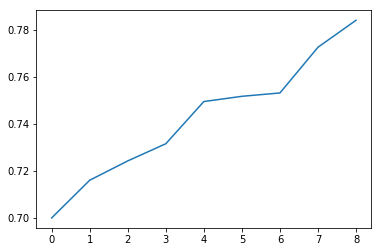
\includegraphics[scale=0.8]{Underlying.png}
\end{figure}

The following plot shows the normalized mean squared error when using different number of trials, starting the iterations from the correct weights. The variance used in the proposal and prior distribution is equal to $0.0001$. The number of iterations was 3000.

\begin{figure}[hbt!]
    \centering
    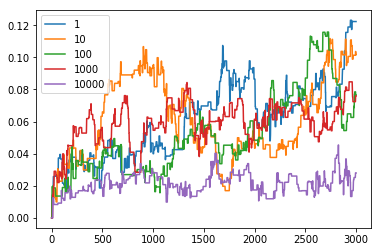
\includegraphics[scale=0.8]{MSE3.png}
\end{figure}

The same was done 100 times for each number of trials. The underlying weights were drawn new for each replicate. The following plot shows the mean of the MSE values at each iteration, with variance bars around it. 

\begin{figure}[hbt!]
    \centering
    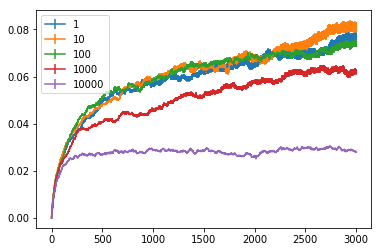
\includegraphics[scale=0.8]{Mean_plot_std.png}
\end{figure}

The standard deviation bars were 

\begin{figure}[hbt!]
    \centering
    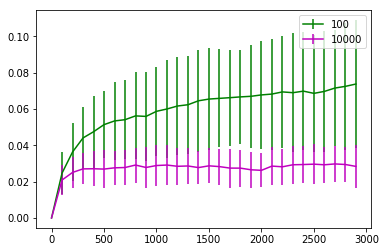
\includegraphics[scale=0.8]{Std_every100.png}
\end{figure}

\textsc{Starting weight trajectory different from true weights}
It is also interesting to see how well the algorithm manages to find the actual weights when the iterations begins from somewhere else. Now the initial guess for the MCMC iterations is set to be a random walk around 1.

\begin{figure}[hbt!]
    \centering
    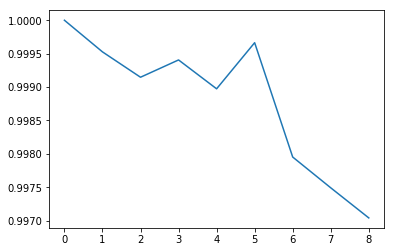
\includegraphics[scale=0.8]{Start_it_1000.png}
\end{figure}


\begin{figure}[hbt!]
    \centering
    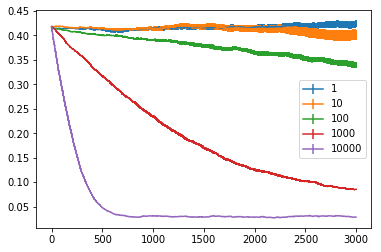
\includegraphics[scale=0.8]{MSE_starting_away.png}
\end{figure}

\subsection{Weights generated by learning rule}

\begin{itemize}
    \item Describe test case and how I generated the weights
    \item Figures with results. Trying different variances for the prior ect
\end{itemize}

\begin{figure}[hbt!]
    \centering
    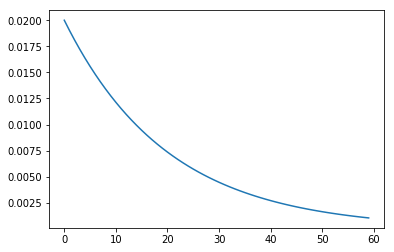
\includegraphics[scale=0.8]{Learning_rule.png}
\end{figure}

\cleardoublepage